\documentclass[10pt,a4paper]{article}
\usepackage[utf8]{inputenc}
\usepackage{amsmath}
\usepackage{amsfonts}
\usepackage{amssymb}
\usepackage[left=2cm,right=2cm,top=2cm,bottom=2cm]{geometry}
\usepackage{url}
\usepackage{graphicx}
\usepackage[per-mode=symbol]{siunitx}

\begin{document}
\title{Task 2: IDEAS Tutorial, part 1}
\author{Filip Jorissen, KU Leuven}
\date{September 20, 2019}
\maketitle

\section*{Introduction}
The goal of this exercise is to become familiar with the 
Modelica package \path{IDEAS.Buildings}. \\

For this exercise you will create a model of a simple house,
using the detailed building envelope component models.
This exercise starts from scratch. 
Model complexity will be increased in each step by 
extending the model from the previous step. 
I.e. for each step (except step 5) a new model should be created that uses
the Modelica \path{extends} clause to extend the previous model.
In between steps, the result differences can be compared.\\


In the following sections the exercise is discussed 
in several steps. 
Each step first qualitatively explains the model part.
Secondly the names of the required IDEAS models 
are listed.
Thirdly we provide high-level instructions of how to
set up the model.
If these instructions are not clear immediately, 
have a look at the model documentation and at the type of
connectors the model has, 
try out some things, 
make an educated guess, etc.
IDEAS.Buildings provides many default parameters that are fine for
this exercise. Notable exceptions to this rule are
the wall type and glazing type of walls and windows, and the zone Medium.
We provide reference results that allow you to check
if your implementation is correct. 
Depending on the parameter values that you choose, results
may differ slightly.
We also list some side notes, which are not strictly required for this
exercise, but which may help you to effectively use Modelica
and IDEAS in the future.

\section{Building  model}
\paragraph{Qualitative discussion}
We will now develop a simple building model that consists of one zone,
four walls, a window and a floor that also serves as a ceiling.
The zone dimensions are 8 m by 4 m and the window is 3 m by 1.4 m. We use the default zone height.
We use double glazing and a heavy wall, meaning they
have high thermal mass.


\paragraph{Required models}
This step requires the main building envelope component models of IDEAS:
\begin{itemize}
\item \path{IDEAS.BoundaryConditions.SimInfoManager}
\item \path{IDEAS.Buildings.Components.Zone}
\item \path{IDEAS.Buildings.Components.OuterWall}
\item \path{IDEAS.Buildings.Components.Window}
\item \path{IDEAS.Buildings.Components.InternalWall}
\end{itemize}

\paragraph{Instructions}
Drag the required components into a newly created model. To inform Modelica how the components are physically `linked', each yellow bus connector of a surface (\path{Window}, \path{OuterWall} or\path{InternalWall}) has to be connected to exactly one zone bus connector.
To support multiple connections, the zone has an array of bus connectors with size \path{nSurf}, where \path{nSurf} is a parameter of \path{Zone}, which has to be set by the user. It is the user's responsibility to ensure that each element of this array is connected to exactly one surface and that there is a total of \path{nSurf} connections to the zone \footnote{While this is quite cumbersome, we will use a more convenient approach later, and automated toolchains are under development to avoid needing this manual indexing.}.

In addition to connecting each surface, the parameters of each component have to be set. 
Components typically have many default values that are appropriate for many purposes.
When parameters do not have a default value, it must be set by the user. 
Notable examples are the \path{Zone} and surface dimensions. 
E.g. \path{inc} and \path{azi} define the surface orientation.
They can be set to a series of predefined constants such as \path{IDEAS.Types.Tilt.Wall}
and \path{IDEAS.Types.Azimuth.S} (S means south).
Furthermore, the zone Medium must be set to \path{IDEAS.Media.Air}.
Glazing and wall types must also be specified.
For this example we propose to use the `BESTEST Heavy Wall' for both the floor and the walls
and a double glazing type, and a south orientation for the window. 


\paragraph{Side notes}
To define the zone geometry, 
we recommend to declare additional parameters such as
\begin{verbatim}
parameter Modelica.SIunits.Length length = 8 "Length of the zone";
\end{verbatim}
and to use these parameters in the zone and surface declaration. 
This improves readability and facilitates changing the building geometry consistently afterwards.\\

Similarly, we recommend to define
\begin{verbatim}
package MediumAir = IDEAS.Media.Air "The air medium";
\end{verbatim}
such that the same medium declaration can be reused for all zones and ventilation components.\\

The \path{SimInfoManager} by default has the modifier \path{inner} in its declaration. 
All IDEAS building components have the modifier \path{outer} in their respective 
declarations of the \path{SimInfoManager}. 
This causes the component declarations to point towards the higher level \path{SimInfoManager}
declaration. This way all model equations for the weather data have to be generated only once,
instead of for each surface.\\

In this simple example we connect both sides of the \path{InternalWall} to the same model.
While this is not physically possible, it's an easy trick to model a building with an 
infinite number of identical zones stacked on top of each other.

\paragraph{Reference result}
We simulate this model with the settings
\begin{enumerate}
\item Start time = 1e7,
\item Stop time = 1.1e7,
\item Number of intervals = 5000.
\end{enumerate}
We thus perform a simulation that starts $10^7$ seconds after new year and ends $10^6$
seconds later, which is a period of 11.6 days.
We now plot the zone temperature, \path{zone.TSensor},
which is the mean of the air temperature and the mean radiative 
temperature of all surfaces, which is indicated in Figure~\ref{fig:res1}.

\begin{figure}
\centering
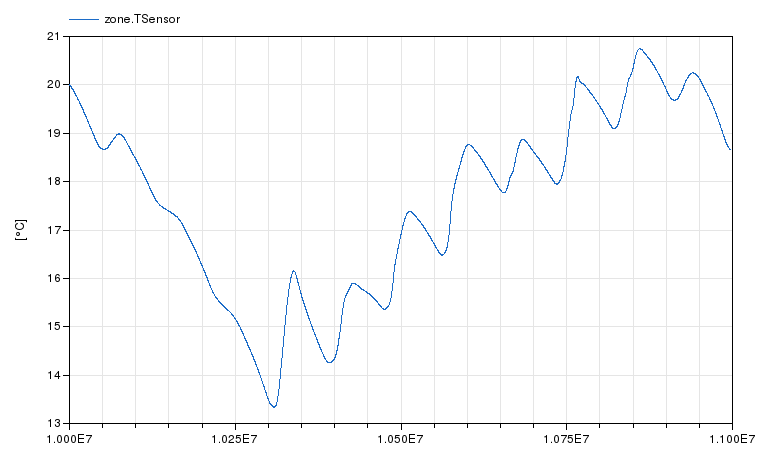
\includegraphics[scale=0.7]{Example1.png}
\caption{The zone temperature as function of time in seconds.}
\label{fig:res1}
\end{figure}


\section{Solar shading extension}
\paragraph{Qualitative discussion}
Modelica supports the notion of `extending' models, which you will
use now to add a screen to the window model.


\paragraph{Required models}
\begin{itemize}
\item \path{Modelica.Blocks.Sources.Constant}
\item \path{IDEAS.Buildings.Components.Shading.Screen}
\end{itemize}

\paragraph{Instructions}
Solar shading is a property of the window and can be chosen using the 
replaceable model `shaType'. 
A drop-down can be opened that lists all available options.
Each option may or may not define custom parameters,
which can be set by pressing the `Edit' button next to the drop-down.

The \path{Screen} model requires an external control signal to define
whether the screen is extended or retracted. 
An input should become visible on the \path{Window} icon for this
purpose. Make sure to connect it to the correct control signal.
See the window input comment for more information on how
to choose the control signal.

\paragraph{Side notes}
The list of available options in the drop-down is automatically generated by
Dymola by scanning all models and by listing all models that extend the partial
that is used in the `constrainedby' clause of the option declaration.


\paragraph{Reference result}
The result with and without the shading model
is plotted in Figure~\ref{fig:res2}.

\begin{figure}
\centering
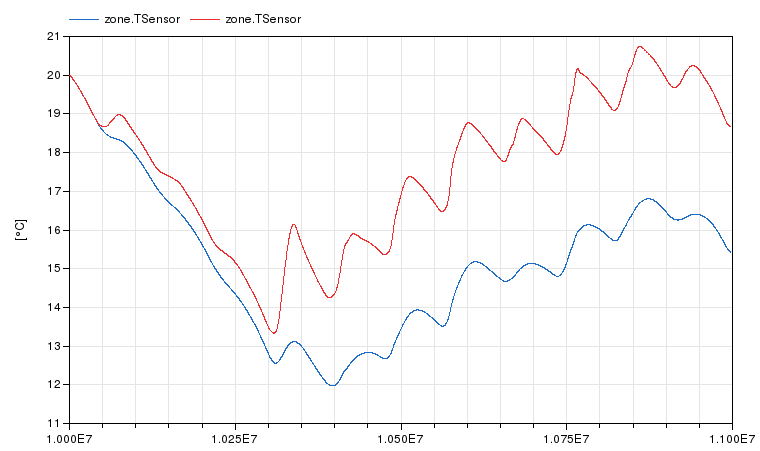
\includegraphics[scale=0.7]{Example2.png}
\caption{Zone temperature with (blue) and without (red) screen model.}
\label{fig:res2}
\end{figure}


\section{Occupancy extension}
\paragraph{Qualitative discussion}
IDEAS has built-in functionalities for zone occupants and lighting.
Based on the chosen options IDEAS will automatically compute
the zone heat gains, relative humidity and CO$_2$ concentration.
Implement a continuous occupancy of 1 person and LED
lighting for the zone by extending the previous model.
The lighting should be on when occupants are present.

\paragraph{Required models}
\begin{itemize}
\item \path{IDEAS.Buildings.Components.Occupants.Fixed}
\item \path{IDEAS.Buildings.Components.LightingType.LED}
\item \path{IDEAS.Buildings.Components.LightingControl.OccupancyBased}
\end{itemize}

\paragraph{Instructions}
Set the appropriate replaceable models in the zone model.

\paragraph{Side notes}
By default, Dymola redeclares models as
\begin{verbatim}
redeclare IDEAS.Buildings.Components.OccupancyType.OfficeWork occTyp,
\end{verbatim}
while it can be advantageous to use
\begin{verbatim}
redeclare replaceable IDEAS.Buildings.Components.OccupancyType.OfficeWork occTyp,
\end{verbatim}
or even
\begin{verbatim}
redeclare replaceable IDEAS.Buildings.Components.OccupancyType.OfficeWork occTyp
  constrainedby IDEAS.Buildings.Components.OccupancyType.OfficeWork(<some options>).
\end{verbatim}
The first alternative allows the model to be replaced once more, 
after having been redeclared a first time and the second option
enforces additional constraints on the second redeclare.
You also have to use the first option in order for the drop-down
to reappear when extending from the model.

\paragraph{Reference result}
The result with and without the occupant and lighting
is plotted in Figure~\ref{fig:res3}.
If you observe no difference between both results, 
it is likely that you forgot to set the number of occupants,
which is an option of \path{IDEAS.Buildings.Components.Occupants.Fixed}
with a default value of 0.


\begin{figure}
\centering
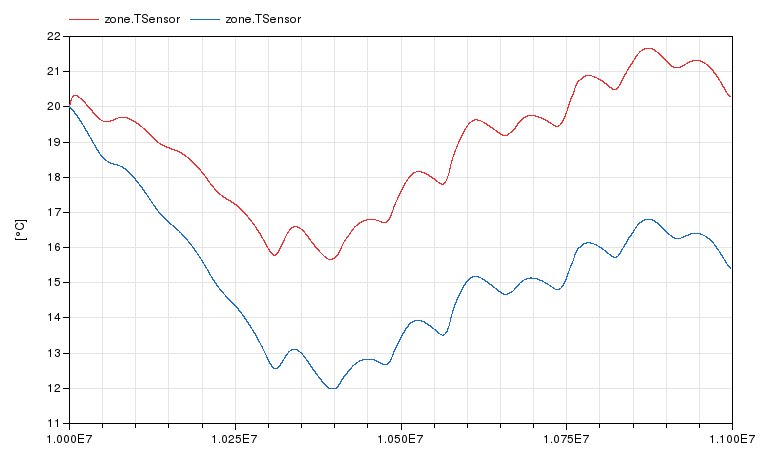
\includegraphics[scale=0.7]{Example3.png}
\caption{Zone temperature with (red) and without (blue) occupant and lighting.}
\label{fig:res3}
\end{figure}


\section{Custom occupancy model}
\paragraph{Qualitative discussion}
The occupancy model that we implemented assumes
that one occupant is continuously present,
which is not realistic.
To get a feeling how replaceable models work,
and how to develop extensions for IDEAS templates,
we will develop and use a new occupancy model
that returns an occupancy of two during
office hours and zero otherwise.

\paragraph{Required models}
\begin{itemize}
\item \path{IDEAS.Buildings.Components.Occupants.BaseClasses.PartialOccupants}
\item \path{IDEAS.Utilities.Time.CalendarTime}
\item \path{Modelica.Blocks.Sources.RealExpression}
\end{itemize}

\paragraph{Instructions}
Create a new model that extends the occupancy model partial.
This partial has an input, which we will not use, and an output, which we have to set.
Create an occupancy signal using a \path{RealExpression} that
returns the parameter value \path{k} during office hours 
(7 - 19 h on week days) and zero otherwise.
Then implement this model by extending the previous example, 
redeclaring the occupancy model and setting parameter $k$.

Hint: use an if-then-else statement (\texttt{if condition then result else other\_result}) with logical checks for the calendar outputs \path{weekDay} and \path{hour}.

\paragraph{Side notes}
The model \path{IDEAS.Buildings.Components.Occupants.BaseClasses.PartialOccupants} 
defines the parameter \path{useInput}.
If this parameter is not fixed, then it will pop up in the parameter window when
setting \path{k}. Since \path{useInput} should not be modified by the end-user,
it is safest to set \path{final useInput=false} in the new occupancy model.
The `final' modifier indicates that the parameter value should no longer be changed
and as such it will no longer be visible to the user in the parameter window.

\paragraph{Reference result}
The result 
is plotted in Figure~\ref{fig:res4}.
Note the much more peaked behaviour of the zone temperature.



\begin{figure}
\centering
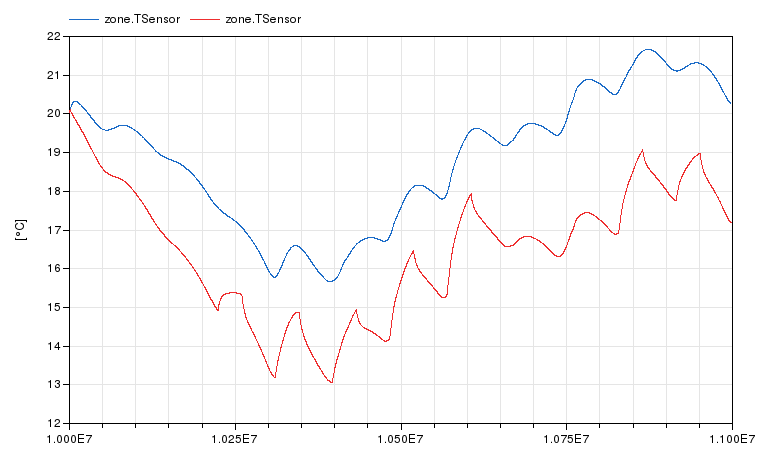
\includegraphics[scale=0.7]{Example4.png}
\caption{Zone temperature with old (blue) and new (red) occupant model.}
\label{fig:res4}
\end{figure}


\section{Split zone model}
\paragraph{Qualitative discussion}
Our building model has only a single zone. 
Furthermore, setting it up is quite involved and requires many connections.
To alleviate this workflow we have developed the model
\path{RectangularZoneTemplate}, which packages a zone, 
windows, walls, a ceiling and a floor and precomputes redundant parameters.
This can significantly reduce implementation work and reduces the chance of making 
errors. 
However, the Modelica specification limits the flexibility that we have to make it really
user-friendly.
This example teaches the use of the \path{RectangularZoneTemplate}.\\

Use \path{RectangularZoneTemplate} to re-create the same building geometry from
step one, this time containing an internal wall that splits the building in two
zones of 4 m x 4 m and with a window on the south and north sides instead of a single window.


\paragraph{Required models}
\begin{itemize}
\item \path{IDEAS.BoundaryConditions.SimInfoManager}
\item \path{IDEAS.Buildings.Components.RectangularZoneTemplate}
\item Construction and glazing records from the first step.
\end{itemize}

\paragraph{Connection instructions}
Create a new model. Add the SimInfoManager and two \path{RectangularZoneTemplate}s.
Set the required parameters in the template, check all tabs! 
Note that the internal wall can only be defined in one of the two templates.
For the other template use an `external connection'. 
The \path{InternalWall} and `external' option will cause a 
yellow bus connector to appear on each of the templates,
which have to be connected to each other.
For the ceiling/floor, apply the same trick.


\paragraph{Reference result}
Figure~\ref{fig:res5} shows the zone temperatures of both zones.
Note the large influence that the window placement has on the zone dynamics!



\begin{figure}
\centering
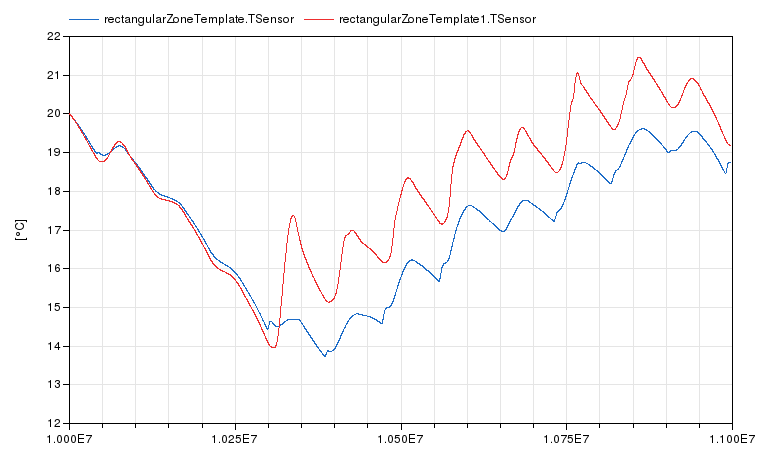
\includegraphics[scale=0.7]{Example5.png}
\caption{Two zone temperatures for step 5.}
\label{fig:res5}
\end{figure}


\end{document}